\Chapter{A MySQL Connector}

\Section{Ismertető}
A MySQL Connector egy MySQL alapú driver JDBC, ODBC, és .NET rendszerek számára. Lehetővé teszi, hogy a fejlesztők adatbázis alkalmazásokat írjanak a támogatott nyelveken. Ezen kívül egy natív C könyvtár teszi lehetővé, hogy a MySQL-t közvetlenül beágyazhassák az alkalmazásaikba.
MySQL által fejlesztett driver -ek:
ADO.NET, ODBC, JDBC, Node.js, Python, C++, C és C API a a klienshez. 
A MySQL közösség által fejlesztetek:
PHP, Perl, Ruby, C+ Wrapper.

*https://www.mysql.com/products/connector/

\Section{A Connector/C++ használata}

Az alábbi weboldalról letöltött állományokat használtam:\newline
https://dev.mysql.com/downloads/connector/cpp/
\begin{itemize}
\item Linux - Generic
\item All
\item Linux - Generic (glibc 2.12) (x86, 64-bit), Compressed TAR Archive
\end{itemize}

Letöltés után kicsomagoljuk. A tartalma egy include és egy lib64 mappa. Az include mappa tartalmát a usr/include könyvtárba másoljuk, a lib64 -ét pedig az usr/lib64 mappába.

Ezután szükség lesz egy külön felhasználóra amellyel a program csatlakozni fog a szerverünkre. Ezt megtehetjük a Workbench alkalmazásban.
\begin{python}
CREATE USER 'newuser'@'localhost' IDENTIFIED BY 'password';
\end{python}

\Section{Első program}

Hozzunk létre egy \texttt{connectortest.cpp} nevű fájlt.
Szükséges osztályok létrehozása:
\begin{cpp}
sql::Driver *driver;
sql::Connection *con;
sql::Statement *stmt;
sql::ResultSet *res;
sql::PreparedStatement *pstmt;
\end{cpp}
Csatlakozás a szerverhez és adatbázis kiválasztása:
\begin{cpp}
driver = get_driver_instance();
con = driver->connect("tcp://192.168.0.43:3306", "program", "a");
con->setSchema("thesis");
\end{cpp}
Utasítás létrehozása SQL parancsból:
\begin{cpp}
pstmt = con->prepareStatement("SELECT * FROM T3");
\end{cpp}
Az utasítás elküldése a szervernek. Ez a sor maga a lekérdezés, itt tudjuk mérni annak idejét is.
\begin{cpp}
res = pstmt->executeQuery();
\end{cpp}
Az eredményt a szemléltetett módon lehet kiolvasni:
\begin{cpp}
 while (res->next())
      cout << res->getInt("c1p3") << "\t" << res->getInt("c2") << "\t"
           << res->getInt("c3") << "\t" << res->getInt("c4") << "\t"
           << res->getInt("fk_p1_p3") << "\t" << res->getInt("fk_p2_p3") 
           << endl;
\end{cpp}


Lekérdezés után fontos törölni az eredményhalmazt és az elkészített utasítást, ugyanis ezek memóriát foglalnak, és több lekérdezés esetén a lekérdezés halmaz megtöltheti a teljes memóriát is. 
\begin{cpp}
    delete res;
    delete pstmt;
\end{cpp}


Futtatáshoz és fordításhoz a következő parancsokat használhatjuk: 
\begin{python}
g++ -D_GLIBCXX_USE_CXX11_ABI=0 connectortest.cpp -o connectortest.out -lmysqlcppconn
./connectortest.out
\end{python}

\Chapter{Párhuzamosítási lehetőségek}

\Section{Az OpenCL nyelv}

Open Computing Language egy keretrendszer amely lehetőséget ad olyan programok írására amelyek különböző platformokon is futtathatóak.
Az OpenCL meghatároz egy programozási nyelvet az eszközök és API-k számára a platformok vezérléséhez és a számítások végrehajtásához az eszközökön. Szabványos interfészt biztosít a párhuzamos számításokhoz, melyhez adatalapú és feladatalapú párhuzamosítást használ.

Fontos észrevenni, hogy az OpenCL natív módon képes beszélni az eszközök nagy részével, ez nem azt jelenti, hogy a kód optimálisan fog futni. Ugyanis különböző Cl eszközök különböző funkciókkal vannak ellátva. Gyártó specifikus kiterjesztések elkerülésével a kód hordozható lesz, de nem sebesség optimális.

\begin{figure}[h!]
\centering
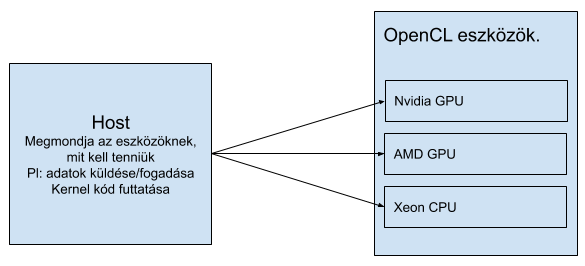
\includegraphics[width=\textwidth]{images/opencl.png}
\caption{OpenCL}
\label{fig:opencl}
\end{figure}

A következő esetekben a GPU-t érdemes használni.
\begin{itemize}
\item Gyors permutáció: Az eszközök gyorsabban mozgatáják a memóriát mint a Host.
\item Adat átváltás: Egyik formátumról másikra.
\item Numerikus gyorsítás: Az eszközök gyorsabban számolnak nagyobb adatdarabokkal mint a Host.
\end{itemize}
Jelen esetben a Host egy asztali számítógép.
Számítási eszközei: CPU, GPU, FPGA, DSP.
A számítási egységek: a magok száma
Elemek feldolgozása: ALU-k magunként.

OpenCL használata mellett szükségtelen gondolkozni azon, hogy pontosan mi is végzi el a számításokat. Ugyanis az OpenCL modelljének illeszkedése egy adott hardverhez, a gyártók feladata.

\begin{table}[h!]
\centering
\caption{CPU-k és GPU-k összehasonlítása}
\medskip
\label{tab:cpuvsgpu}
\begin{tabular}{|p{7cm}|p{7cm}|}
\hline
Alacsony számítási sűrűség & Magas számítási sűrűség \\
\hline
Komplex logikai vezérlő & Magas számítási és memória-hozzáférés \\
\hline
Nagy caches &   \\
\hline
Optimalizált a soros műveletekre.
\begin{itemize}
	\item Kevesebb végrehajtási egység (ALU).
	\item Magas órajel sebesség.
\end{itemize} & Beépített párhuzamos műveletek.
\begin{itemize}
	\item Sok párhuzamos végrehajtási egység (ALU).
	\item A grafika a párhuzamosság legismertebb esete.
\end{itemize} \\
\hline
Shallow pipelines <30 stages & Deep pipelines több száz szakasz \\
\hline
Alacsony késleltetési tolerancia & Magas áteresztőképesség, Magas áteresztőképesség \\
\hline
Az újabb CPU-k több párhuzamosításra képesek & Újabb GPU-k
\begin{itemize}
	\item Jobb áramlást vezérlő logika
	\item Scatter/Gather Memory Access
	\item Már nem egyirányúak a pipeline-ok
\end{itemize} \\
\hline
\end{tabular}
\end{table}

\Section{Az OpenCL elemei}
\SubSection{Eszköz modell}

\begin{figure}[h!]
\centering
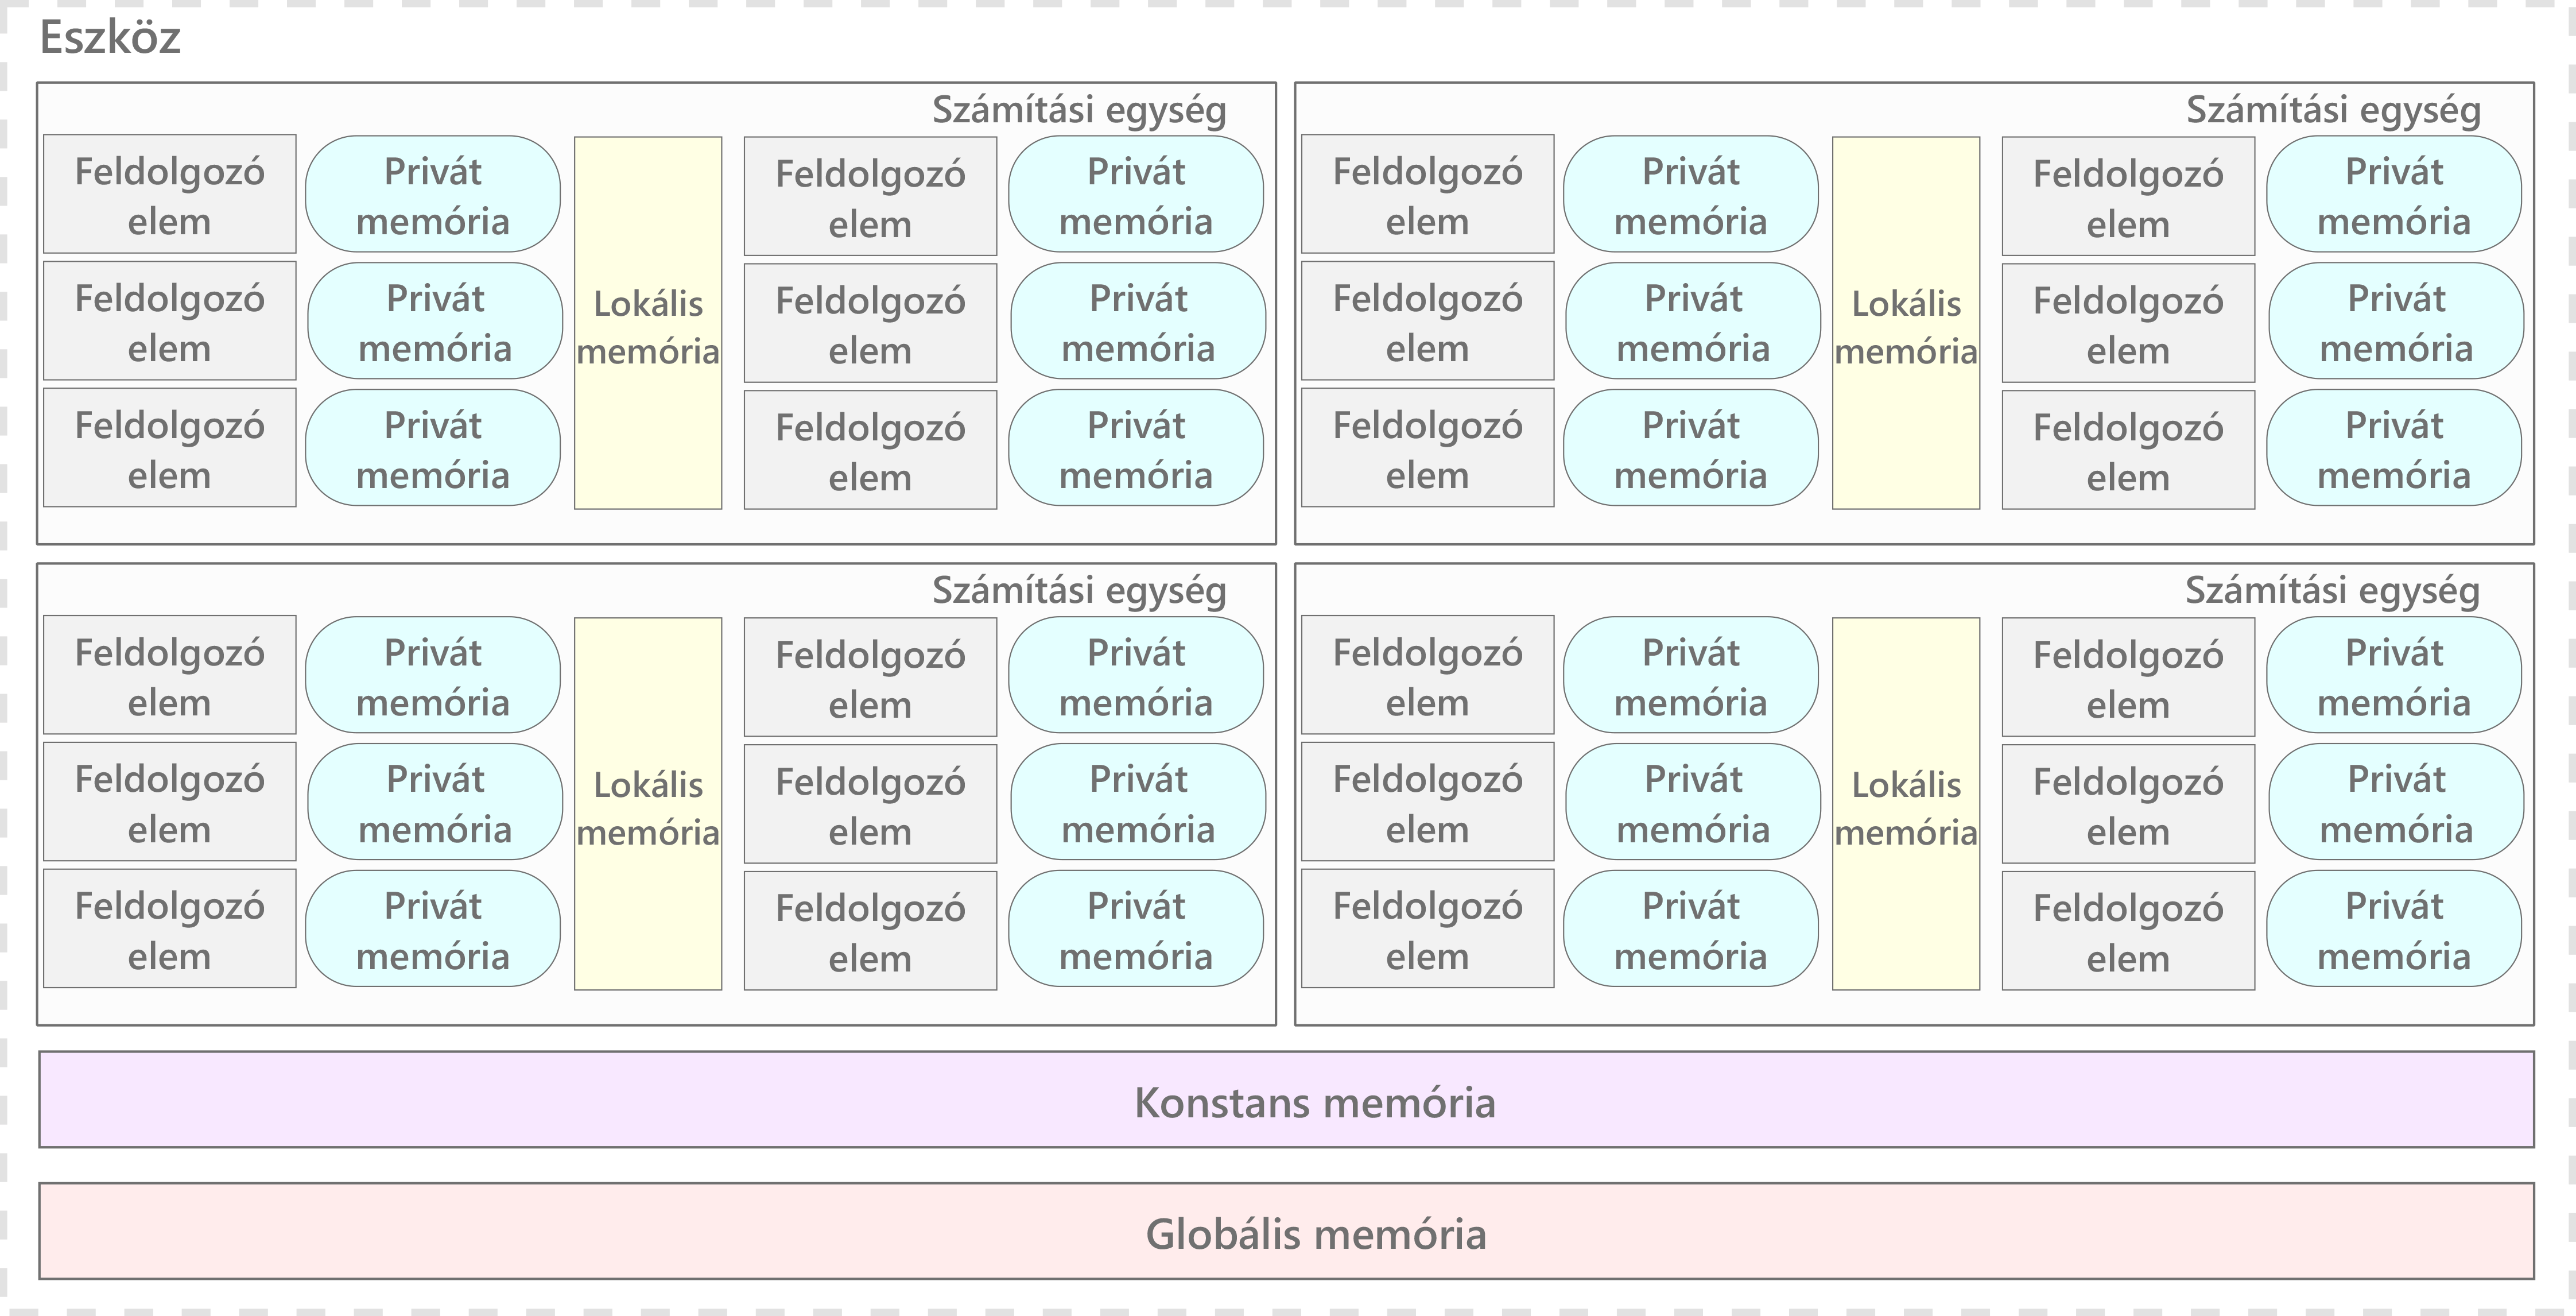
\includegraphics[width=\textwidth]{images/device.png}
\caption{OpenCL eszköz modell}
\label{fig:opencl}
\end{figure}

Négy féle memóriát különböztetünk meg:
\begin{itemize}
\item Globális memória: Minden eszközzel meg van osztva, de lassú. A kernel hívások között perzisztens. 
\item Konstans memória: Gyorsabb a globálisnál, szűrő paraméterek megadására használják.
\item Lokális memória: Minden számási egység számára privát, de megosztott a feldolgozó elemek között.
\item Privát memória: Gyorsabb a lokálisnál, minden feldolgozó elemnek van.
\end{itemize} 
A konstans, lokális és privát memóriába nem lehet adatokat menteni úgy, hogy más kernel használhassa majd azt

\SubSection{Feldolgozási modell}

A Host -on OpenCL alkalmazások futnak amelyek a számítási eszközökhöz küldik a munkát.
\begin{itemize}
\item Munkaelem: A számítási eszköz alapvető egysége.
\item Kernel: A kód, ami fut a munkaegységen  (Alap C függvények)
\item Program: Kernelek és egyéb funkciók gyűjteménye
\item Kontextus: A környezet a munkaelemek végrehajtásához. (Eszközök, annak memóriái és parancssorai)
\item Parancssor: Sor melyet a Host arra használ, hogy a munkát (Kernelek, memória másolatok) az eszközbe küldje.
\end{itemize}

Ez egy keretrendszer, amely meghatározza, hogy a kernel hogyan hajtsa végre a probléma egyes pontjait. Vagy hogyan bontsa a feladatot munka elemekre.

Amire ehhez szükség van:
\begin{itemize}
\item Globális munkaméret. Ez általában egy bemeneti vektor teljes hossza.
\item Globális eltolás.
\item Munkacsoport méret.
\end{itemize}

Megfeleltetés:
\begin{itemize}
\item Munkaelem - számítási elem: Minden munkaelemet egy számítási elem hajt végre.
\item Munkacsoport - számítási egység: Minden munkacsoportot egy számítási egység hajt végre. A munkacsoport munkaelemek, a számítási egység pedig számítási elemek csoportja.
\item Kernel végrehajtási példány - Számítási eszköz. Munkacsoportok összessége illetve számítási elemek összessége. 
\end{itemize}

\SubSection{Munkacsoportok}

Ideális esetben végtelen számú feldolgozási elemmel rendelkezik az eszköz, Minden ilyen elem az adatok egy részét kezeli anélkül, hogy szükségük lenne kommunikációra. De ez nem így szokott lenni, ezért a munkát fel kell osztani.
\begin{itemize}
\item A teljes munkát fel kell osztani kisebb darabokra.
\item Minden darab egy munkacsoporthoz tartozik.
\item A munkacsoportokat ütemezéssel kell végrehajtani a számítási egységeken.
\item Minden csoport rendelkezik egy megosztott memóriával, ami olyan mint a lokális memória a számítási-egységeknél
\end{itemize}

A folytatáshoz a munkacsoportokat ütemezni kell a végrehajtási egységeken, és a munkaelemeket számítási-egységen belül végrehajtani.
Minden munkaelem társulni fog egy számítási egységhez, ha van elegendő. Ezt a folyamatot az OpenCL végzi, csak meg kell adni a globális munkaméretet és munkacsoport méretet. A kernelt indító függvény a  munkacsoportok számát kiszámolja. Ha nincs elég számítási egység, akkor a munkacsoportok sorban hajtódnak végre a meglévő egységeken.

\SubSection{OpenCL program általános felépítése}
\begin{itemize}
\item Definiálni kell a platformot és a parancssort.
\item Definiálni kell a szükséges memória objektumokat.
\item Létre kell hozni a programot a szövegből.
\item Fel kell építeni a programot.
\item Létre kell hozni a kernelt és be kell állítani a paramétereit.
\item Futtatni kell a kernel kódot.
\item Ki kell olvasni a memóriaobjektumokban található választ a Host-on.

\end{itemize}


\Section{Az OpenCL telepítése}

A megfelelő működéshez az első lépést már a rendszer telepítésénél megtettem amikor a non-free avagy az nvidia eredeti drivernének a telepítését választottam.
ezen kívül a következő csomagokra volt szükség: 

\begin{python}
$ sudo pacman -S opencl-headers
$ sudo pacman -S opencl-nvidia
$ sudo pacman -S cuda
$ sudo pacman -S ocl-icd
\end{python}

\Section{Az OpenCL használata}

\Chapter{Megvalósítás}
\Section{Bevezetés}
Az alap ötlet egyszerű. A MySQL szerverről lekérjük a tábla tartalmát, amit be másolunk az OpenCL pufferébe, majd a kernelkód futtatása után az eredményt tartalmazó részeket kiolvassuk. De felvetődik pár problémás rész. Hogyan tároljuk a tábla tartalmát? Mekkora legyen a Globális munkaméret és a munkacsoport méret? Milyen formában állítsuk elő az eredményt, és hogyan olvassuk azt ki?

\SubSection{Táblák tömbbé alakítása}
Ahhoz, hogy OpenCL el kezelni tudjuk az adatokat először szükség lesz egy struktúrára ami reprezentálja az adatbázis tábla felépítését. Az az a struktúra adattagjainak típusa egyezzen meg a táblázat oszlopainak típusával. Ezek után ebből létre kell hoznunk egy tömböt melynek hossza legalább annyi, mint a tábla sorainak száma.

\begin{figure}[h!]
\centering
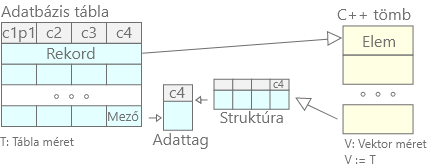
\includegraphics[width=10cm]{images/table-struct.png}
\caption{Adatbázistábla átalakítása tömbbé}
\label{fig:opencl}
\end{figure}

\begin{itemize}
\item A struktúra megfelel a tábla felépítésének.
\item A tömb egy eleme, egy ilyen struktúra.
\item A tömb egy eleme megfelel a tábla egy rekordjának azaz sorának.
\item Egy elem adattagjai megfelelnek az adatbázis egyazon rekordjához tartozó mezőknek.
\end{itemize}

\newpage
\SubSection{A táblákat beolvasó függvény.}

A táblák sorainak száma változó lehet, ezért a programot igyekeztem úgy megírni, hogy alkalmazkodjon közel bármilyen táblamérethez.
Első lépésben létrehozok egy Pointert ami a táblára fog mutatni, és ehhez egy változót ami a méretét tárolja. Az adatbázis lekérő függvénynek átadom ezeket.
Miután a Connector elvégezte a lekérdezést beállítom a méret változó értékét és a tábla memória területét csak ekkor foglalom le. A kettős indirektségnek köszönhetően a főprogramban lévő *t1 pointer beállítható, hogy a megfelelő címre mutasson, illetve a függvényből feltölthető.
\begin{cpp}
Table1Type *t1 = NULL;
int t1_size;
load_database(&t1, &t1_size);
	
res = pstmt->executeQuery();
\end{cpp}
\begin{figure}[h!]
\centering
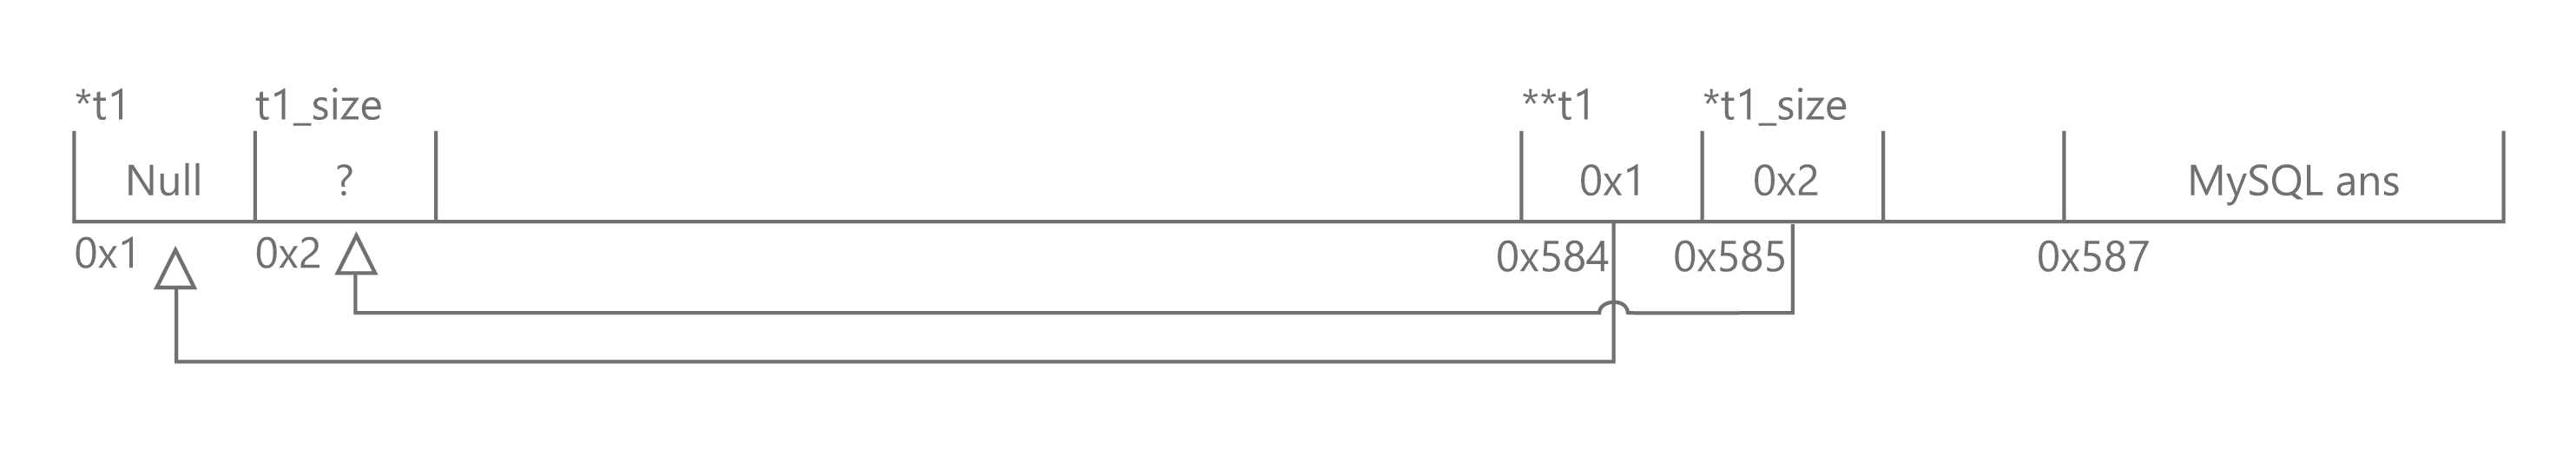
\includegraphics[width=\textwidth]{images/pointer1.png}
\caption{Pointerek a létrehozáskor}
\label{fig:opencl}
\end{figure}

\begin{cpp}
int i = 0;
*T1_size = res->rowsCount();
*T1 = (Table1Type*) malloc(sizeof(Table1Type) * *T1_size);

while (res->next())
{
	T1[0][i].c1p1 = res->getInt("c1p1");
	T1[0][i].c2 = res->getInt("c2");
	T1[0][i].c3 = res->getInt("c3");
	T1[0][i].c4 = res->getInt("c4");
	i++;
}
\end{cpp}

\begin{figure}[h!]
\centering
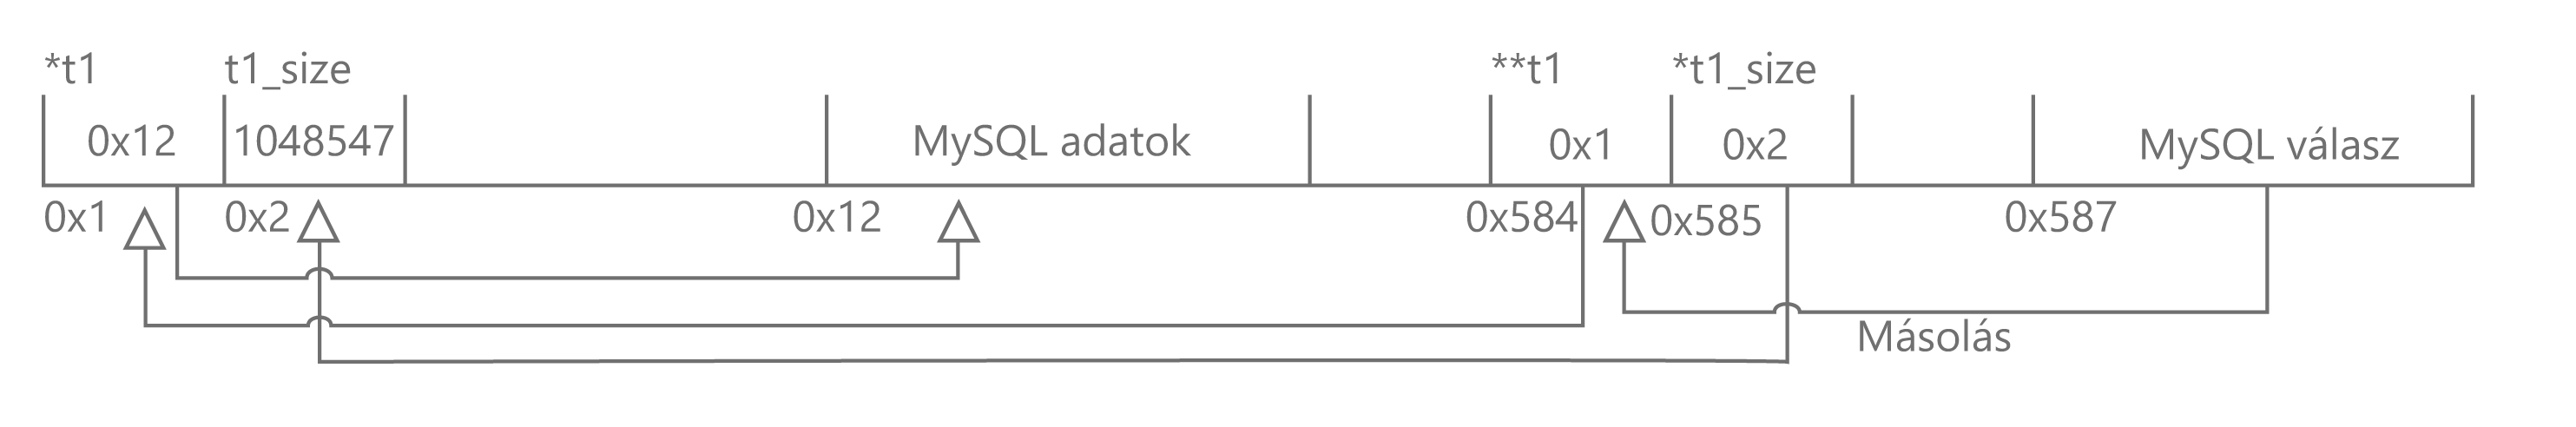
\includegraphics[width=\textwidth]{images/pointer2.png}
\caption{Pointerek teljes működése}
\label{fig:opencl}
\end{figure}

\Section{Globális és lokális méret meghatározása}
\begin{itemize}
\item Ennél a pontnál oda kell figyelni pár alapvető dologra.
\item A globális méret korlátlan.
\item A lokális méret avagy munkaelemek száma egy munkacsoportban legfeljebb, 1024 lehet.
\item A lokális méret osztója kell, hogy legyen a globális méretnek.
\item A túl sok vagy túl kevés munkacsoport használata esetén a párhuzamosság előnye elveszhet.
\item A munkacsoportok párhuzamosan dolgoznak egymás mellett.
\item Munkacsoporton belül a munkaelemek feldolgozása párhuzamos.
\item Munkacsoportok között nincs szinkronizáció, csak munka elemek között, ha egy munkacsoportba tartoznak.
\item Nem használható kölcsönös kizárás, a szemafor végtelen ciklust okoz.
\end{itemize}

\SubSection{Alap működés}

Alap esetben a bemeneti elemszámot megadjuk globális méretnek, gyakorlatilag ennyiszer fog lefutni a kernel kód.
Megadjuk a lokális méretet, ezzel munkacsoportokba bontottuk az elemeket.
A végeredményt tartalmazó kimeneti vektor hossza egyezik a globális mérettel, így nem ütközhetünk bele abba a hibába, hogy két számítási elem ugyan oda próbáljon írni. Amennyiben például a 545. elem megfelel, akkor az indexe és egyéb hozzá tartozó értékek az 545. helyen lesznek a kimeneti tömbben.

\begin{figure}[h!]
\centering
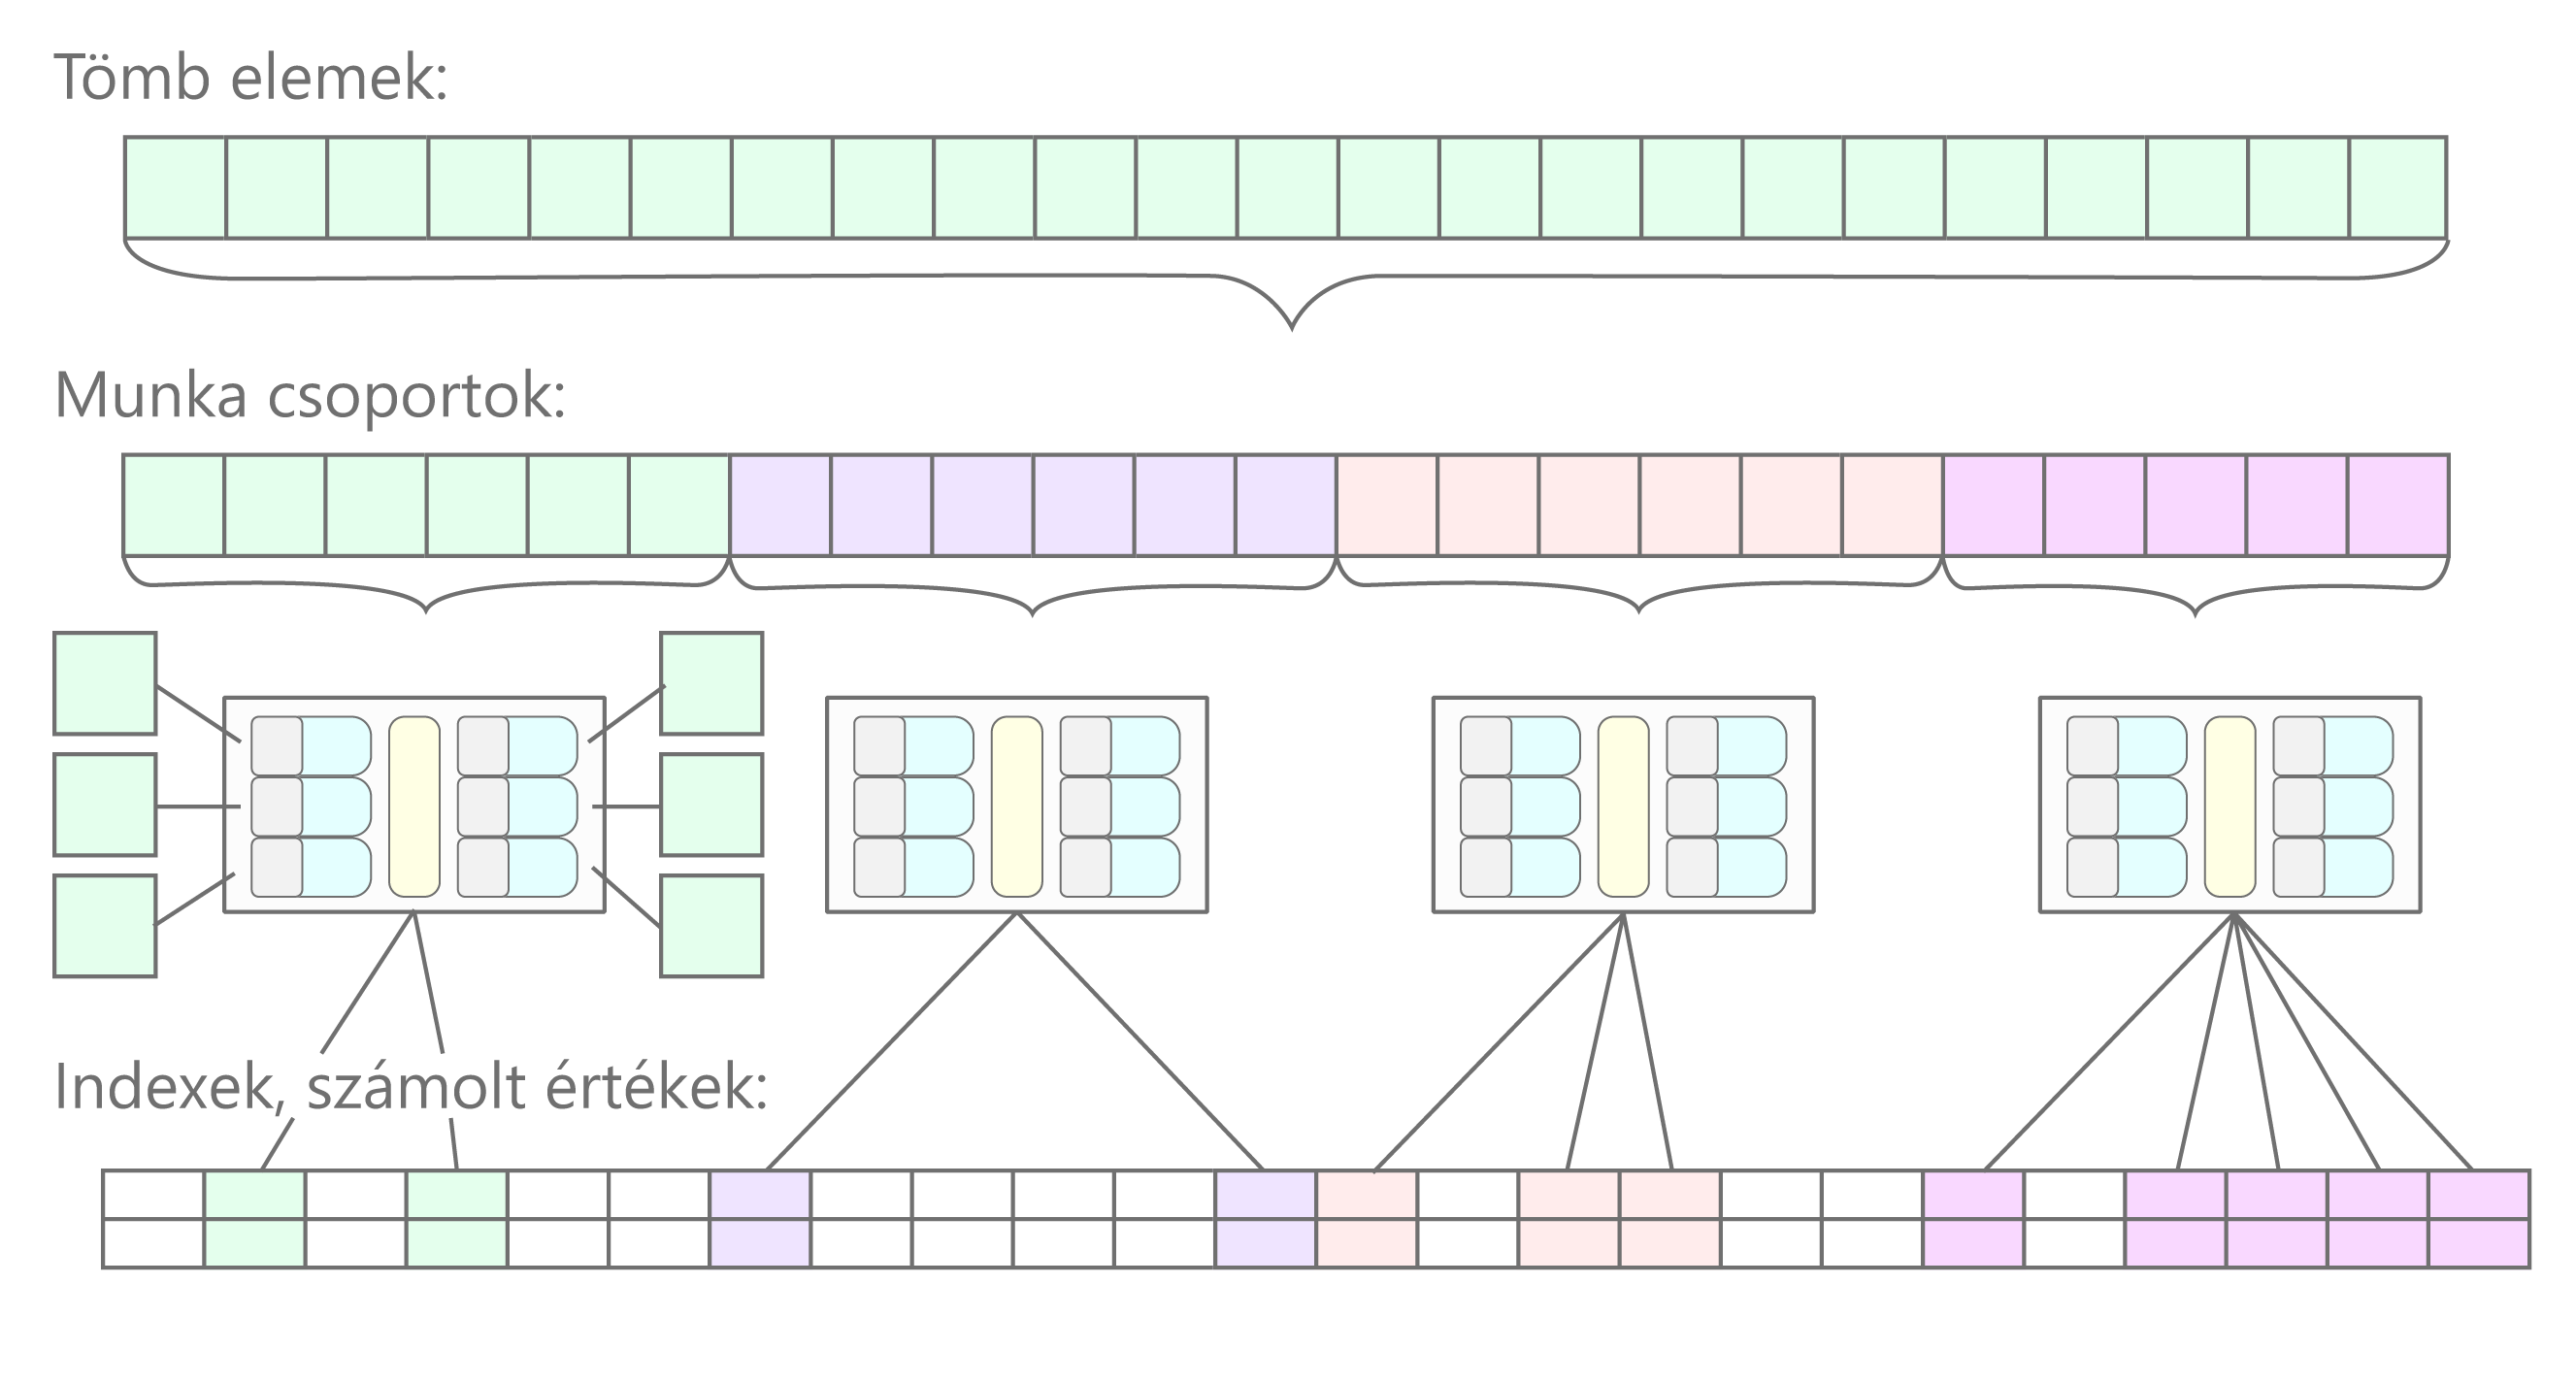
\includegraphics[width=\textwidth]{images/workgroups.png}
\caption{Munkacsoportokra bontás}
\label{fig:opencl}
\end{figure}

\SubSection{Globális méret meghatározása}
Tegyünk fel, hogy kaptunk egy 1048547 sorból álló táblázatot.
Olyan lokális méretet kell megadni, ami ennek osztója, láthatjuk, hogy a meghatározása problémás.
Erre megoldást jelent ha a lokális méretet előre beállítjuk például 1024 -re, majd a globális méretet ebből és a sorok számából kiszámítjuk.
Ezt úgy tehetjük meg, hogy a sorok számához hozzáadjuk a legkisebb olyan számot amellyel az összeg oszthatóvá válik a lokális mérettel.
Így azt kapjuk, hogy a globális méret 1049600, ami azt jelenti, hogy 1025 munkacsoport jön létre. 

Viszont látjuk, hogy a lokális méret korlátai miatt szükség lehet arra, hogy valamilyen egyéb módon csökkentsük a munkacsoportok számát.
Mondjuk azt, hogy egy munkaegység ne csak egy elemén dolgozzon a tömbnek, hanem egy intervallumán.
Határozzuk meg a méreteket a következők alapján:

$$ interval\_size = \floor{ \sqrt{table\_size} } $$
$$global\_size = interval\_size + ( local\_size - (interval\_size\mod(local\_size)) )$$

Ezzel elértük, hogy a munkacsoportok száma drasztikusan csökkenjen. Illetve egy másik fontos előnyre is szert ettünk, ami az eredmények számlálása illetve kiolvasása során lesz jelentős.

\SubSection{A kernelkód működése}

Annak köszönhetően, hogy a tömböt intervallumokra bontottuk az elemeire nézve soros feldolgozási darabok jöttek létre. Ezeken az intervallumokon már 
használhatunk számlálókat. Ennek az lesz a következménye, hogy nem csak a kimeneti tömböt kell kiolvasni, aminek mérete továbbra is megegyezik a táblázat sorainak számával, de a számlálókat tartalmazó tömböt is.
De vegyük észre, hogy legfeljebb csak a gyökével nőtt az eredetileg kiolvasandó méret, és a kimeneten pontosan tudjuk, hol vannak az adatok.

\begin{figure}[h!]
\centering
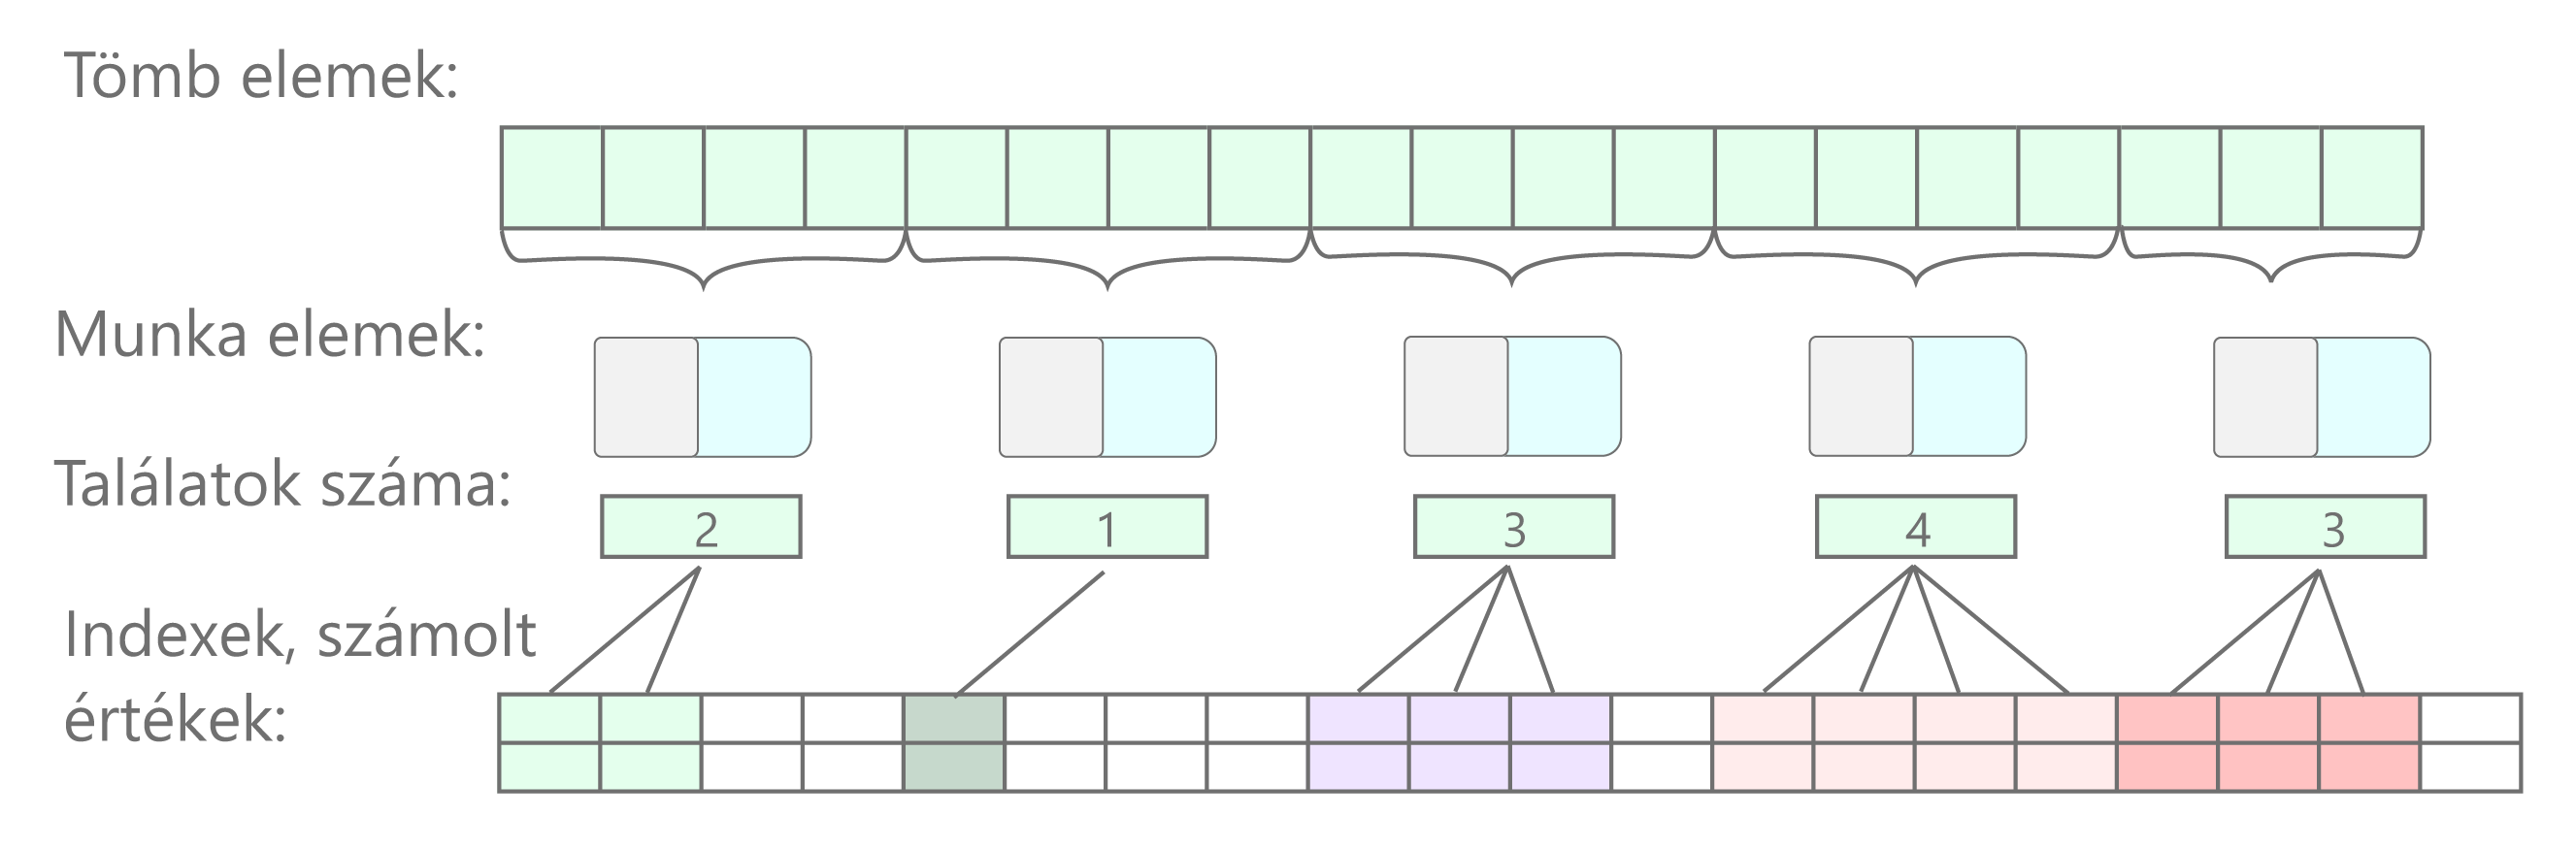
\includegraphics[width=\textwidth]{images/itemgroup.png}
\caption{Munkacsoportokra bontás}
\label{fig:opencl}
\end{figure}

A számítási elemek egy intervallumon dolgoznak és továbbra is munkacsoportokba vannak bontva de ez a működésre nincs hatással, legfeljebb a teljesítményre.

\SubSection{Az elemek kiolvasása}
Meglehet tenni azt, hogy nem olvassuk ki azonnal a végeredményt tartalmazó tömböt.
Első lépésben kiolvassuk a számlálókat, ezt végig járva az eredmény tömbből kiolvashatjuk csak azokat a részeket amelyek ténylegesen
tartalmaznak indexeket. 
Később látni fogjuk, hogy ez a módszer mégsem olyan hatékony mint első ránézésre gondolnánk.


\begin{figure}[h!]
\centering
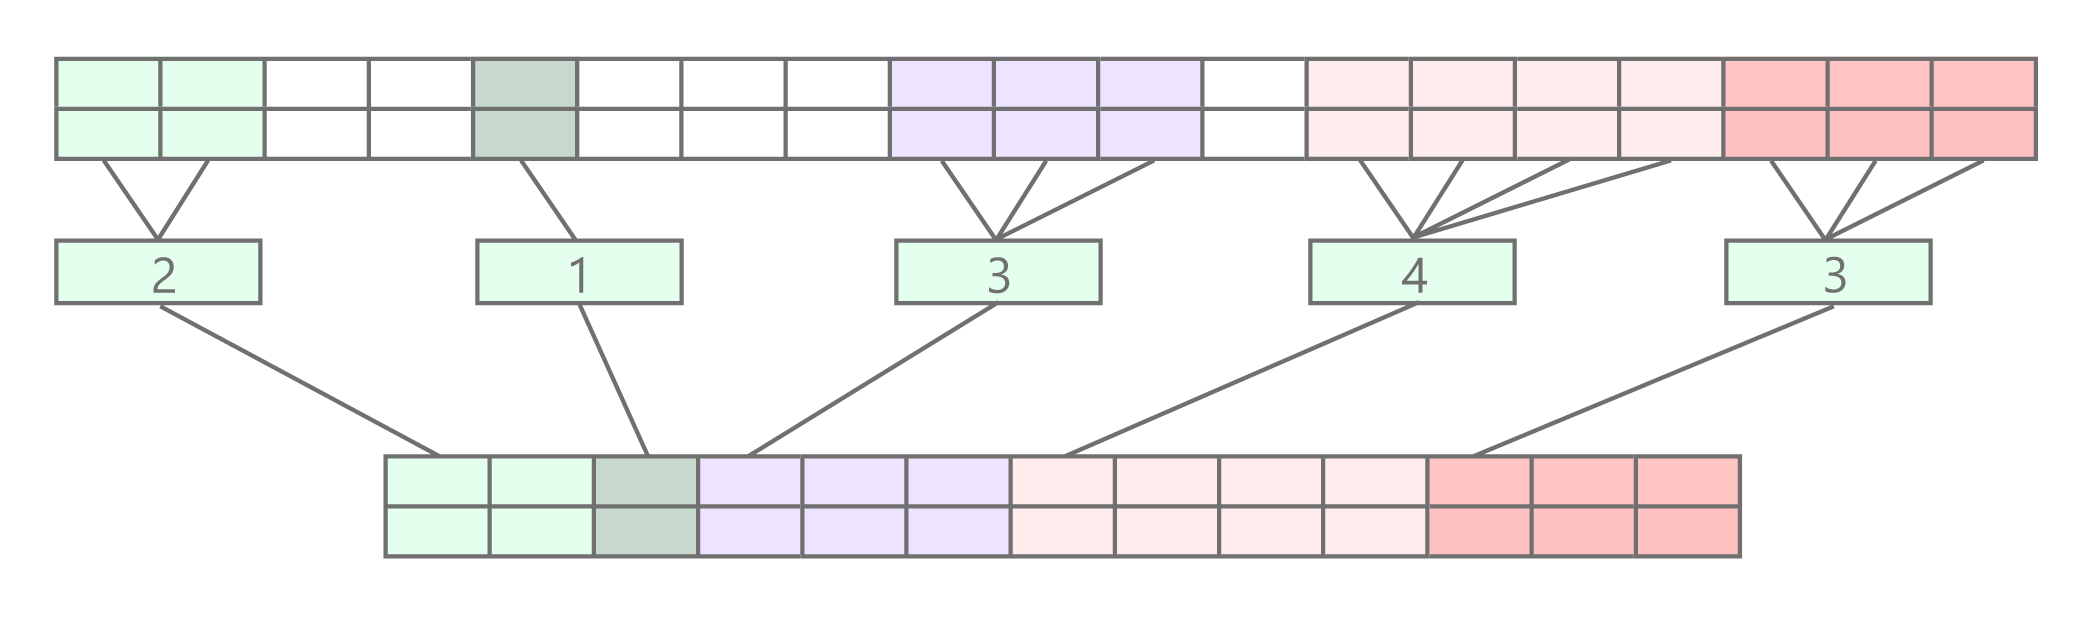
\includegraphics[width=\textwidth]{images/kimasol.png}
\caption{Munkacsoportokra bontás}
\label{fig:opencl}
\end{figure}




